\documentclass[letWterpaper,10pt,titlepage]{article}

\usepackage{graphicx}
\usepackage{amssymb}
\usepackage{amsmath}
\usepackage{amsthm}
\usepackage{alltt}
\usepackage{float}
\usepackage{color}
\usepackage{url}
\usepackage{balance}
\usepackage[TABBOTCAP, tight]{subfigure}
\usepackage{enumitem}
\usepackage{pstricks, pst-node}
\usepackage{geometry}
\geometry{textheight=10in, textwidth=7.5in}
\newcommand{\cred}[1]{{\color{red}#1}}
\newcommand{\cblue}[1]{{\color{blue}#1}}
\usepackage{hyperref}
\usepackage{textcomp}
\usepackage{listings}

%% The following metadata will show up in the PDF properties
\hypersetup{
  colorlinks = true,
  urlcolor = black,
  pdfkeywords = {cs325 ``Analysis of Algorithms'' subarray sum},
  pdftitle = {CS325 Project 1},
  pdfsubject = {CS325 Project 1},
  pdfpagemode = UseNone
}

\definecolor{comment}{rgb}{0, 0.6, 0}

\lstset{
    belowcaptionskip=1\baselineskip,
    breaklines=true,
    frame=single,
    xleftmargin=\parindent,
    language=Python,
    showstringspaces=false,
    basicstyle=\footnotesize\ttfamily,
    identifierstyle=\color{blue},
    stringstyle=\color{orange},
    commentstyle=\color{comment},
}

\parindent = 0.0 in
\parskip = 0.2 in


\begin{document}

\title{CS 325 Project 1: Maximum Sum Subarray}
\author{Project Group 25:\\Jonathon Moore\\Jaden Diefenbaugh\\Kenneth Hafdahl}
\maketitle

\section{Theoretical Run-time Analysis}

\subsection{Enumeration}

\begin{lstlisting}
def maxSumSubarray(array):
    bestSum = array[0]
    #lower index of max sum array
    bestLower = 0
    #upper index of max sum array
    bestUpper = 0
    for n in range(len(array)):
        for m in range(n, len(array)):
            currentSum = 0
            for p in range(n, m+1):
                currentSum = currentSum + array[p]
            if currentSum > bestSum:
               bestSum = currentSum
               bestUpper = m
               bestLower = n
\end{lstlisting}

The first two loops of the enumeration algorithm determine the starting and ending indices of the subarray to be summed. There is one subarray of length $n$ generated, two arrays of length $n-1$, three arrays of length $n-2$, and so on. This totals $1, 2, 3, ..., n={n(n+1)}/2$ arrays which is $\Theta(n^2)$ complexity. The innermost loop sums the values between the two indices to determine if the current array is the maximum sum subarray. This is an $\Theta(n)$ operation that is performed for each of the subarrays, making this algorithm $\Theta(n^3)$.

\subsection{Better Enumeration}

\begin{lstlisting}
def maxSumSubarray(array):
    bestSum = array[0]
    #lower index of max sum array
    bestLower = 0
    #upper index of max sum array
    bestUpper = 0
    currentSum = 0
    for n in range(len(array)):
        lastSum = 0
        for m in range(n, len(array)):
            if m == n:
               currentSum = array[n]
            else:
                currentSum = lastSum + array[m]
            lastSum = currentSum
            if currentSum > bestSum:
               bestSum = currentSum
               bestUpper = m
               bestLower = n
\end{lstlisting}

The next version of the enumeration method removes the innermost addition loop. This is achieved by keeping a running sum for each subarray. The sum is resent when the lower bound is increased and the size of the array is zero. This optimization allows the algorithm to achieve a $\Theta(n^2)$ complexity.

\subsection{Divide and Conquer}

\begin{lstlisting}
# the combining half of algorithm3
def mergeHalves(lowerHalf, upperHalf):
    #set bounds of new combined array
    j = lowerHalf[0]
    k = upperHalf[1]

    #compute max sum of combined arrays
    # it will either be:
    #   the max sum of lowerHalf
    #   the max sum of upperHalf
    #   the combined sums upper end of lowerHalf and lower end of upperHalf
    if lowerHalf[2] > upperHalf[2]:
        newMaxSum = lowerHalf[2]
        maxSumJ = lowerHalf[3]
        maxSumK = lowerHalf[4]
    else:
        newMaxSum = upperHalf[2]
        maxSumJ = upperHalf[3]
        maxSumK = upperHalf[4]
    suffixMaxSum = lowerHalf[7] + upperHalf[5]
    if suffixMaxSum > newMaxSum:
        newMaxSum = suffixMaxSum
        maxSumJ = lowerHalf[8]
        maxSumK = upperHalf[6]

    return [j, k, newMaxSum, maxSumJ, maxSumK, -1, -1, -1, -1]


# recursive solution to finding the max sum (algorithm 3)
def algorithm3(array, lower, upper):
    upperSum = [];
    lowerSum = [];
    # format of array that holds return data:
    # Bounds of subarray:
    # [0] lower bound of subarray
    # [1] upper bound of subarray
    # MaxSum data within that array:
    # [2] bestMaxSum
    # [3] lower bound of range that holds bestMaxSum
    # [4] upper bound of range that holds bestMaxSum
    # Best sum that overlaps along the lower bound of subarray:
    # [5] bestMaxSum that includes lower bound of the subarray
    # [6] upper bound of the range that creates bestMaxSum(Lower)
    # Best sum that overlaps along the upper bound of subarray:
    # [7] bestMaxSum that includes upper bound of the subarray
    # [8] lower bound of the range that creates bestMaxSum(Upper)
    bestMaxSum = [lower, upper, -99999, 0, 0, -99999, 0, -99999, 0]
    if lower == upper:  #size of subarray is 1
        bestMaxSum = [lower, upper, array[lower], lower, upper, array[lower], lower, array[upper], upper]
    else:   # split array into 2 subarrays and recursively merge their answers
        mid = math.floor((upper + lower) / 2)
        lowerSum = algorithm3(array, lower, mid)
        upperSum = algorithm3(array, mid+1, upper)
        bestMaxSum = mergeHalves(lowerSum, upperSum)


        #find best sum that covers the lower suffix of the joined array
        best_here = 0
        best_so_far = 0
        best_pos = 0

        for i in range(bestMaxSum[0], bestMaxSum[1]+1):
            best_here = array[i] + best_here
            if best_here > best_so_far:
                best_so_far = best_here
                best_pos = i

        bestMaxSum[5] = best_so_far
        bestMaxSum[6] = best_pos

        #find best sum that covers the upper suffix of the joined array
        best_here = 0
        best_so_far = 0
        best_pos = 0
        for j in range(bestMaxSum[1], bestMaxSum[0]-1, -1):
            best_here = array[j] + best_here
            if best_here > best_so_far:
                best_so_far = best_here
                best_pos = j

        bestMaxSum[7] = best_so_far
        bestMaxSum[8] = best_pos

    return bestMaxSum
\end{lstlisting}

The divide and conquer approach is a recursive algorithm that has a base case in which the size of the subarray is 1. If the subarray size is greater than 1, a midpoint is calculated for the divide and the algorithm is recursively called on either half. A helper function is then called that logically merges the two halves. The each subarray has a maximum sum sequence and two maximum sum sequences that start or end on the subarray bounds. If the combination of two subarrays yields a summation that is larger than either if the individual summations, that merge is returned. The division portion of the algorithm is $O(log_2(n))$ and the merging portion is $O(1)$. However, the portion determining the maximum arrays of the subsection are still $O(n^2)$, meaning that this algorithm has the same complexity.

\subsection{Linear-Time}

\begin{lstlisting}
def maxSumSubarray(array):
    sbustSum = array[0]
    bestLower = currLower = 0
    bestUpper = currUpper = 0
    currentSum = array[bestLower]

    if len(array) > 1:
        #loop through all values, appending each to the "array of solved max"
        for i in range(1, len(array)):
            if array[i] > curentSum + array[i]:
                currLower = i
                currUpper = i
                currentSum = array[i]
            else:
                currUpper = i
                currentSum += array[i]

            if currentSum > bestSum:
                bestLower = currLower
                bestUpper = currUpper
                bestSum = currentSum
\end{lstlisting}

The linear-time implementation has a single loop that steps through the elements of the array. Each iteration contains work that is constant time since only simple comparisons are made, so the complexity of this algorithm is $O(n)$.

\section{Proof of Correctness}

\section{Testing}
We tested the validity of our algorithms by running each implementation with an input of MSS\_Problems.txt. This file contains an array per line that consists of positive and negative integers. Our test.py program reads in these arrays and stores the corresponding output to MSS\_Solutions.txt where the subarray indices are listed in addition to the maximum sum found. Each of the algorithm implementations produced the same output, suggesting a correct implementation. Trivial input examples where there is a single positive value, all positive values, or an array with a length of one all return correct results on visual inspection.

\section{Experimental Analysis}

\begin{figure}
    \centering
    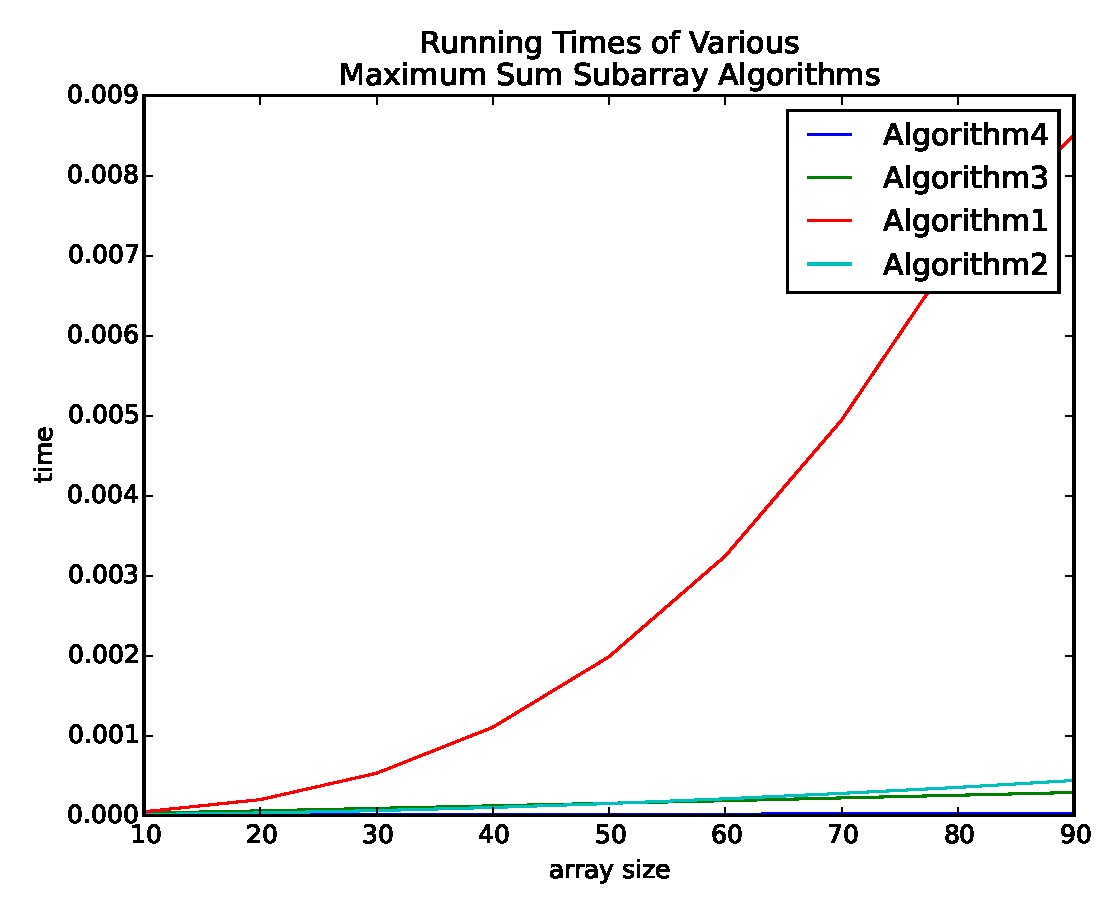
\includegraphics[width=0.75\textwidth]{../bin/testrun.eps}
\end{figure}

The figure below displays the performance time of each algorithm as the size of the array grows. The line of best fit for the first and second algorithms is a polynomial of degree 2. The third and fourth Algorithms both have lines of best fit that is linear. However, algorithm 4 growds significantly slower than the divide and conquer algorithm.

\section{Extrapolation and Interpretation}
\begin{center}
    \begin{tabular}{|l|c|r|}
        \hline
        Algorithm & Trendline & Inverse \\ \hline
        1 & $2\times10^{-6}x^2-7\times10^{-5}x+0.0007$ & $17.5+2.5\sqrt{80000x-7}$\\ \hline
        2 & $2\times10^{-8}x^2+6\times10^{-7}x+7\times10^{-6}$ & $-5+\frac{5\sqrt{2000000x-11}}{\sqrt{3}}$\\ \hline
        3 & $4\times10^{-6}x-6\times10^{-6}$ & $250000(x+6)$ \\ \hline
        4 & $3\times10^{-7}x+6\times10^{-6}$ & $\frac{20}{3}(500000x-3)$ \\ \hline
    \end{tabular}
\end{center}

The graph above shows the equations for the trendlines that match the graphed data. The inverse provides a function $f(x)$ that returns the number of elements required to fill $x$ seconds worth of computation time. Plugging one hour (3600 seconds) into each of the inverse functions reveals how large of an array each of the algorithms can handle in that time.

\begin{center}
    \begin{tabular}{|l|c|r|}
        \hline
        Algorithm & Array Size \\ \hline
        1 & $42443$ \\ \hline
        2 & $244944$ \\ \hline
        3 & $901500000$ \\ \hline
        4 & $1.2\times10^{10}$ \\ \hline
    \end{tabular}
\end{center}

\end{document}
